\chapter{Probability}

\section{Basic Concepts}
\begin{definition}[Experiment]
    An experiment is any process that can be repeated and has a well-defined set of possible outcomes.
\end{definition}

\begin{definition}[Sample Space $S$]
    The sample space \( S \) of an experiment is the set of all possible outcomes of that experiment.
\end{definition}

\begin{definition}[Event]
    An event is any subset of the sample space \( S \). An event occurs if the outcome of the experiment is an element of that subset.
\end{definition}

\begin{eg}
    When throwing a pair of dice, the sample space is:
    \[
        S = \{(1,1), (1,2), \ldots, (6,6)\}
    \]
    An example event $E$ could be "the sum of the two dice is 3", then the set of outcomes in $E$ is:
    \[
        E = \{(1,2), (2,1)\}
    \]
    Thus the event $E$ occurs if the outcome of the experiment is either (1,2) or (2,1).
\end{eg}

\section{Laplace Definition of Probability}
\begin{definition}[Laplace]
    The Laplace definition of probability states that if all outcomes in the sample space are equally likely, the probability of an event \( E \) is given by:
    \[
        P(E) = \frac{|E|}{|S|}
    \]
    where \( |E| \) is the number of outcomes in event \( E \) and \( |S| \) is the total number of outcomes in the sample space.
\end{definition}

\begin{eg}
    Continuing with the previous example of throwing a pair of dice, the total number of outcomes in the sample space is \( |S| = 36 \). The event \( E \) (sum of the two dice is 3) has \( |E| = 2 \) outcomes. Therefore, the probability of event \( E \) occurring is:
    \[
        P(E) = \frac{|E|}{|S|} = \frac{2}{36} = \frac{1}{18}
    \]
\end{eg}

\begin{eg}
    If two dices are rolled after each other, what is the probability to roll at least one 6? \\
    Let $E$ be the event "at least one 6 is rolled", the the possible outcome set is:
    \[
        E = \{(6, 1...6), (1...6, 6)\}
    \]
    By the principle of inclusion-exclusion, we have:
    \[
        |E| = 6 + 6 - 1 = 11
    \]
    More explicitly:
    \[
        E = \{(6,1), (6,2), (6,3), (6,4), (6,5), (6,6), (1,6), (2,6), (3,6), (4,6), (5,6)\}
    \]
    Thus the probability of rolling at least one 6 is:
    \[
        P(E) = \frac{|E|}{|S|} = \frac{11}{36}
    \]
\end{eg}

\begin{theorem}
    Let $E$ be an event in the sample space $S$. The probability of the event $\bar{E} = S - E$, the complementary event of $E$, is given by:
    \[
        P(\bar{E}) = 1 - P(E)
    \]
\end{theorem}
\begin{proof}
    Since \( E \) and \( \bar{E} \) are complementary events, we have:
    \[
        |S| = |E| + |\bar{E}|
    \]
    Dividing both sides by \( |S| \), we get:
    \[
        1 = \frac{|E|}{|S|} + \frac{|\bar{E}|}{|S|}
    \]
    Therefore:
    \[
        P(E) + P(\bar{E}) = 1
    \]
    Rearranging gives:
    \[
        P(\bar{E}) = 1 - P(E)
    \]
\end{proof}

\begin{eg}
    A sequence of 10 bits is chosen randomly. What is the probability that at least one of these bits is 0? \\
    Let $E$ be the event "at least one bit is 0". The complementary event $\bar{E}$ is "all bits are 1". There is only one outcome in $\bar{E}$, which is the sequence "1111111111". The total number of possible outcomes in the sample space is \( |S| = 2^{10} = 1024 \). Thus, the probability of the complementary event is:
    \[
        P(\bar{E}) = \frac{1}{1024}
    \]
    Therefore, the probability of event \( E \) occurring is:
    \[
        P(E) = 1 - P(\bar{E}) = 1 - \frac{1}{1024} = \frac{1023}{1024}
    \]
\end{eg}

\begin{theorem}
    Let $E_1$ and $E_2$ be two events in the sample space $S$. The probability of the union of the two events is given by:
    \[
        P(E_1 \cup E_2) = P(E_1) + P(E_2) - P(E_1 \cap E_2)
    \]
\end{theorem}
\begin{proof}
    By the principle of inclusion-exclusion, we have:
    \[
        |E_1 \cup E_2| = |E_1| + |E_2| - |E_1 \cap E_2|
    \]
    Dividing both sides by \( |S| \), we get:
    \[
        \frac{|E_1 \cup E_2|}{|S|} = \frac{|E_1|}{|S|} + \frac{|E_2|}{|S|} - \frac{|E_1 \cap E_2|}{|S|}
    \]
    Therefore:
    \[
        P(E_1 \cup E_2) = P(E_1) + P(E_2) - P(E_1 \cap E_2)
    \]
\end{proof}

\begin{eg}
    What is the probability that a positive integer selected at random from the set of positive integers not exceeding $100$ is divisible by $2$ or $5$? \\
    Let $E_1$ be the event "the number is divisible by 2" and $E_2$ be the event "the number is divisible by 5". We have:
    \[
        |E_1| = 50, \quad |E_2| = 20, \quad |E_1 \cap E_2| = 10
    \]
    The total number of outcomes in the sample space is \( |S| = 100 \). Therefore, the probabilities are:
    \[
        P(E_1) = \frac{50}{100} = \frac{1}{2}, \quad P(E_2) = \frac{20}{100} = \frac{1}{5}, \quad P(E_1 \cap E_2) = \frac{10}{100} = \frac{1}{10}
    \]
    Using the formula for the union of two events, we have:
    \[
        P(E_1 \cup E_2) = P(E_1) + P(E_2) - P(E_1 \cap E_2) = \frac{1}{2} + \frac{1}{5} - \frac{1}{10} = \frac{5}{10} + \frac{2}{10} - \frac{1}{10} = \frac{6}{10} = \frac{3}{5}
    \]
\end{eg}

\subsection{Limitation of the Laplace Definition}
The Laplace definition of probability is limited to situations where all outcomes in the sample space are equally likely. In many real-world scenarios, this assumption does not hold true, and outcomes may have different probabilities of occurring. In such cases, more advanced probability theories and models, such as Bayesian probability or frequentist probability, are used to accurately represent and analyze the likelihood of events.

\section{Probability Distributions}
\begin{definition}[Probability Distribution]
    Let $S$ be a sample space of an experiment with a finite or countable number of outcomes. Each outcome $s$ is assigned a probability $P(s)$ such that:
    \begin{itemize}[itemsep=1pt,label=$\circ$]
        \item $0 \leq P(s) \leq 1$ for every outcome $s$ in $S$.
        \item The sum of the probabilities of all outcomes in $S$ is equal to 1:
        \[
            \sum_{s \in S} P(s) = 1
        \]
    \end{itemize}
    The function $P: S \to [0, 1]$ that assigns probabilities to outcomes is called a probability distribution.
\end{definition}

\begin{eg}
    Probability distribution for the sum of two rolling dice. The set of possible outcomes for the sum ranges from 2 to 12, thus $S = \{2, 3, 4, 5, 6, 7, 8, 9, 10, 11, 12\}$. The probabilities for each possible sum are not equal, as some sums can be achieved through multiple combinations of dice rolls, for example:
    \begin{itemize}[itemsep=1pt,label=$\circ$]
        \item Sum of 2: (1,1) $\to$ 1 way
        \item Sum of 3: (1,2), (2,1) $\to$ 2 ways
        \item Sum of 4: (1,3), (2,2), (3,1) $\to$ 3 ways
        \item $\ldots$
        \item Sum of 7: (1,6), (2,5), (3,4), (4,3), (5,2), (6,1) $\to$ 6 ways
        \item $\ldots$
        \item Sum of 12: (6,6) $\to$ 1 way
    \end{itemize}
    There are a total of 36 possible outcomes when rolling two dice. Therefore, the probabilities for each sum can be calculated as the number of ways to achieve that sum divided by 36, for example:
    \[
        P(2) = \frac{1}{36}, \quad P(3) = \frac{2}{36}, \quad P(4) = \frac{3}{36}, \quad \ldots
    \]
\end{eg}

\begin{eg}
    What probabilities should we assign to the outcomes $H$ (heads) and $T$ (tails) when the coin is biased so that heads come up twice as often as tails? \\
    Let $P(T) = x$. Since heads come up twice as often as tails, we have $P(H) = 2x$. According to the properties of probability distributions, we have:
    \[
        P(H) + P(T) = 1
    \]
    Substituting the values, we get:
    \[
        2x + x = 1 \quad \implies \quad 3x = 1 \quad \implies \quad x = \frac{1}{3}
    \]
    Therefore, the probabilities are:
    \[
        P(T) = \frac{1}{3}, \quad P(H) = \frac{2}{3}
    \]
\end{eg}

\begin{definition}[Uniform Distribution]
    Suppose that $S$ is a set with $n$ elements. The uniform distribution assigns the probability \( \frac{1}{n} \) to each element of \( S \). In other words, for every outcome \( s \) in \( S \):
    \[
        P(s) = \frac{1}{n}
    \]
\end{definition}

\begin{definition}[Probability of an Event]
    Let \( E \) be an event in the sample space \( S \) with a probability distribution \( P \). The probability of the event \( E \) is given by:
    \[
        P(E) = \sum_{s \in E} P(s)
    \]
    where the sum is taken over all outcomes \( s \) that belong to the event \( E \).
\end{definition}

\begin{eg}
    Suppose that a die is biased so that $3$ appears twice as often as any other number, but that the other five outcomes are equally likely. What is the probability that an odd number is rolled? \\
    Let $P(1) = P(5) = P(2) = P(4) = P(6) = x$ and $P(3) = 2x$. According to the properties of probability distributions, we have:
    \[
        P(1) + P(2) + P(3) + P(4) + P(5) + P(6) = 1
    \]
    Substituting the values, we get:
    \[
        x + x + 2x + x + x + x = 1 \quad \implies \quad 7x = 1 \quad \implies \quad x = \frac{1}{7}
    \]
    Therefore, the probabilities are:
    \[
        P(1) = P(5) = P(2) = P(4) = P(6) = \frac{1}{7}, \quad P(3) = \frac{2}{7}
    \]
    The event "rolling an odd number" consists of the outcomes \( \{1, 3, 5\} \). Thus, the probability of rolling an odd number is:
    \[
        P(\{1, 3, 5\}) = P(1) + P(3) + P(5) = \frac{1}{7} + \frac{2}{7} + \frac{1}{7} = \frac{4}{7}
    \]
\end{eg}

\begin{theorem}
    The probability of the complement of an event \( E \) in a sample space \( S \) with a probability distribution \( P \) is given by:
    \[
        P(\bar{E}) = 1 - P(E)
    \]
\end{theorem}
\begin{proof}
    Since \( E \) and \( \bar{E} \) are complementary events, we have:
    \[
        S = E \cup \bar{E} \quad \text{and} \quad E \cap \bar{E} = \emptyset
    \]
    Therefore, the probability of the sample space is:
    \[
        P(S) = P(E) + P(\bar{E}) = 1
    \]
    Rearranging gives:
    \[
        P(\bar{E}) = 1 - P(E)
    \]
\end{proof}

\begin{theorem}
    Let $E_1$ and $E_2$ be two events in the sample space $S$ with a probability distribution $P$. The probability of the union of the two events is given by:
    \[
        P(E_1 \cup E_2) = P(E_1) + P(E_2) - P(E_1 \cap E_2)
    \]
\end{theorem}
\begin{proof}
    By the principle of inclusion-exclusion, we have:
    \[
        P(E_1 \cup E_2) = P(E_1) + P(E_2) - P(E_1 \cap E_2)
    \]
\end{proof}

\begin{theorem}
    If $E_1, E_2, \ldots, E_n$ are mutually exclusive events in the sample space $S$ with a probability distribution $P$, then the probability of the union of these events is given by:
    \[
        P\left(\bigcup_{i=1}^{n} E_i\right) = \sum_{i=1}^{n} P(E_i)
    \]
\end{theorem}

\section{Conditional Probability}
\begin{definition}[Conditional Probability]
    The conditional probability of an event \( A \) given that another event \( B \) has occurred is denoted by \( P(A|B) \) and is defined as:
    \[
        P(A|B) = \frac{P(A \cap B)}{P(B)} \quad \text{provided that } P(B) > 0
    \]
\end{definition}

\begin{eg}
    When you roll a dice, what is the probability that the outcome is even?
    \begin{itemize}[itemsep=1pt,label=$\circ$]
        \item Without any additional knowledge, the probability is:
        \[
            P(\text{even}) = \frac{3}{6} = \frac{1}{2}
        \]
        \item If we know that the outcome is less than or equal to 3, then the possible outcomes are \( \{1, 2, 3\} \). The only even number in this set is 2. Therefore, the conditional probability is:
        \[
            P(\text{even} | \text{outcome} \leq 3) = \frac{\frac{1}{6}}{\frac{1}{2}} = \frac{1}{3}
        \]
    \end{itemize}
\end{eg}

\begin{eg}
    When you toss a coin $6$ times, what is the probability that the last toss is heads?
    \begin{itemize}[itemsep=1pt,label=$\circ$]
        \item Without any additional knowledge, the probability is:
        \[
            P(H) = \frac{2^5}{2^6} = \frac{1}{2}
        \]
        \item If we know that the first $5$ tosses were all heads. We have that:
        \[
            E \cap F = \{(H, H, H, H, H, H)\}
        \]
        and:
        \[
            F = \{(H, H, H, H, H, H), (H, H, H, H, H, T)\}
        \]
        Thus:
        \[
            P(F) = \frac{2^1}{2^6} = \frac{1}{2^5}
        \]
        Therefore, the conditional probability is:
        \[
            P(E|F) = \frac{P(E \cap F)}{P(F)} = \frac{\frac{1}{2^6}}{\frac{1}{2^5}} = \frac{1}{2}
        \]
    \end{itemize}
\end{eg}

\begin{definition}[Independent Events]
    Two events \( A \) and \( B \) are said to be independent if the occurrence of one event does not affect the probability of the occurrence of the other event. Mathematically, this is expressed as:
    \[
        P(A|B) = P(A) \quad \text{or equivalently} \quad P(B|A) = P(B)
    \]
    This can also be expressed in terms of joint probability:
    \[
        P(A \cap B) = P(A) \cdot P(B)
    \]
\end{definition}

\begin{eg}
    If $P(E) = \frac{1}{2}$ and $P(E \cap F) = \frac{1}{4}$ under which condition are $E$ and $F$ independent? \\
    By the definition of independent events, we have:
    \[
        P(E \cap F) = P(E) \cdot P(F)
    \]
    Substituting the given values, we get:
    \[
        \frac{1}{4} = \frac{1}{2} \cdot P(F) \quad \implies \quad P(F) = \frac{1}{2}
    \]
\end{eg}

\begin{eg}
    Assume that each of the four ways that a family can have two children is equally likely: $\{GG, GB,BG,BB\}$. Are the events $E$ that a family with two children has both girls and boys and $F$ that a family with two children has at most one boy, independent? \\
    We have:
    \[
        E = \{GB, BG\}, \quad F = \{GG, GB, BG\}
    \]
    Thus:
    \[
        P(E) = \frac{2}{4} = \frac{1}{2}, \quad P(F) = \frac{3}{4}
    \]
    and:
    \[
        E \cap F = \{GB, BG\}
    \]
    Therefore:
    \[
        P(E \cap F) = \frac{2}{4} = \frac{1}{2}
    \]
    Now, we check if:
    \[
        P(E) \cdot P(F) = \frac{1}{2} \cdot \frac{3}{4} = \frac{3}{8} \neq P(E \cap F)
    \]
    Since \( P(E) \cdot P(F) \neq P(E \cap F) \), the events \( E \) and \( F \) are not independent.
\end{eg}

\begin{definition}[Pairwise Independent Events]
    A set of events \( E_1, E_2, \ldots, E_n \) are said to be pairwise independent if every pair of events \( (E_i, E_j) \) for \( i \neq j \) are independent. This means that for every pair \( (E_i, E_j) \):
    \[
        P(E_i \cap E_j) = P(E_i) \cdot P(E_j)
    \]
\end{definition}

\begin{definition}[Mutually Independent Events]
    A set of events \( E_1, E_2, \ldots, E_n \) are said to be mutually independent if for every subset of events \( \{E_{i_1}, E_{i_2}, \ldots, E_{i_k}\} \) where \( 2 \leq k \leq n \), the following condition holds:
    \[
        P(E_{i_1} \cap E_{i_2} \cap \ldots \cap E_{i_k}) = P(E_{i_1}) \cdot P(E_{i_2}) \cdot \ldots \cdot P(E_{i_k})
    \]
\end{definition}
Remark that mutual independence implies pairwise independence, but the converse is not necessarily true.

\begin{eg}
    Toss a fair coin twice with a sample space:
    \[
        S = \{HH, HT, TH, TT\}
    \]
    With the events:
    \begin{itemize}[itemsep=1pt,label=$\circ$]
        \item $E_1$ = "first toss is heads" = $\{HH, HT\}$
        \item $E_2$ = "second toss is heads" = $\{HH, TH\}$
        \item $E_3$ = "the two outcomes are different" = $\{HT, TH\}$
    \end{itemize}
    We have:
    \[
        P(E_1) = P(E_2) = P(E_3) = \frac{1}{2}
    \]
    And:
    \[
        P(E_1 \cap E_2) = P(\{HH\}) = \frac{1}{4} = P(E_1) \cdot P(E_2)
    \]
    \[
        P(E_1 \cap E_3) = P(\{HT\}) = \frac{1}{4} = P(E_1) \cdot P(E_3)
    \]
    \[
        P(E_2 \cap E_3) = P(\{TH\}) = \frac{1}{4} = P(E_2) \cdot P(E_3)
    \]
    Thus, the events \( E_1, E_2, E_3 \) are pairwise independent. However:
    \[
        P(E_1 \cap E_2 \cap E_3) = P(\emptyset) = 0 \neq P(E_1) \cdot P(E_2) \cdot P(E_3) = \frac{1}{8}
    \]
    Therefore, the events \( E_1, E_2, E_3 \) are not mutually independent.
\end{eg}

\begin{eg}
    Consider the following:
    \begin{itemize}[itemsep=1pt,label=$\circ$]
        \item Two dice are tossed remotely.
        \item An observer tells you a preperty of the rolls.
        \item Depending on the answer, you decide whether you bet that the sum of the two dice is $7$.
    \end{itemize}
    Let's first check the case where the observer does not tell you anything. The possible outcomes for the sum of two dice are:
    \[
        E = \{16, 25, 34, 43, 52, 61\}
    \]
    Thus, the probability of getting a sum of $7$ is:
    \[
        P(E) = \frac{6}{36} = \frac{1}{6}
    \]
    Now, let's consider the case where the observer tells you that at least one of the dice shows a $6$. The possible outcomes are:
    \[
        F = \{(6,1), (6,2), (6,3), (6,4), (6,5), (6,6), (1,6), (2,6), (3,6), (4,6), (5,6)\}
    \]
    with:
    \[
        P(F) = \frac{11}{36}
    \]
    And:
    \[
        E \cap F = \{(6,1), (1,6)\} \quad \implies \quad P(E \cap F) = \frac{2}{36}
    \]
    Therefore, the conditional probability of getting a sum of $7$ given that at least one die shows a $6$ is:
    \[
        P(E|F) = \frac{P(E \cap F)}{P(F)} = \frac{\frac{2}{36}}{\frac{11}{36}} = \frac{2}{11}
    \]
    Which is greater than the initial probability of \( \frac{1}{6} \).
\end{eg}

\begin{definition}[Bernoulli Trial]
    A Bernoulli trial is a random experiment that has exactly two possible outcomes, typically referred to as "success" and "failure". The probability of success is denoted by \( p \), and the probability of failure is denoted by \( q = 1 - p \).
\end{definition}
A frequent question regarding Bernoulli trials is: If we perform \( n \) mutually independent Bernoulli trials, what is the probability of getting exactly \( k \) successes?

\begin{eg}
    A coin is biased such that the probability of heads is \( \frac{2}{3} \) and the probability of tails is \( \frac{1}{3} \). What is the probability that exactly $4$ heads occur when the coin is flipped $7$ times? \\
    Let \( p = \frac{2}{3} \) be the probability of heads and \( q = \frac{1}{3} \) be the probability of tails. The number of ways to choose \( 4 \) heads out of \( 7 \) flips is given by the binomial coefficient \( \binom{7}{4} \). The probability of getting exactly \( 4 \) heads is given by:
    \[
        P(X = 4) = \binom{7}{4} p^4 q^{7-4} = \binom{7}{4} \left(\frac{2}{3}\right)^4 \left(\frac{1}{3}\right)^3
    \]
\end{eg}

\begin{theorem}[Independent Bernoulli Trials]
    If a Bernoulli trial with probability of success \( p \) is repeated \( n \) times independently, the probability of getting exactly \( k \) successes is given by:
    \[
        P(X = k) = \binom{n}{k} p^k (1 - p)^{n - k}
    \]
\end{theorem}
\begin{proof}
    The number of ways to choose \( k \) successes out of \( n \) trials is given by the binomial coefficient \( \binom{n}{k} \). Each specific sequence of \( k \) successes and \( n - k \) failures has a probability of \( p^k (1 - p)^{n - k} \). Therefore, the total probability of getting exactly \( k \) successes is:
    \[
        P(X = k) = \binom{n}{k} p^k (1 - p)^{n - k}
    \]
\end{proof}
Remark that the sum of the probabilities for all possible values of \( k \) (from \( 0 \) to \( n \)) is equal to \( 1 \):
\[
    \sum_{k=0}^{n} P(X = k) = \sum_{k=0}^{n} \binom{n}{k} p^k (1 - p)^{n - k} = (p + (1 - p))^n = 1^n = 1
\]

\begin{eg}
    When planting $7$ seeds, what's the probability that at least $3$ will sprout, if each seed has a $25\%$ chance of sprouting? \\
    Let \( p = 0.25 \) be the probability of a seed sprouting and \( q = 0.75 \) be the probability of a seed not sprouting. The probability of at least \( 3 \) seeds sprouting is given by:
    \[
        P(X \geq 3) = 1 - P(X < 3) = 1 - (P(X = 0) + P(X = 1) + P(X = 2))
    \]
    We calculate each term:
    \[
        P(X = 0) = \binom{7}{0} (0.25)^0 (0.75)^7 = (0.75)^7
    \]
    \[
        P(X = 1) = \binom{7}{1} (0.25)^1 (0.75)^6 = 7 \cdot 0.25 \cdot (0.75)^6
    \]
    \[
        P(X = 2) = \binom{7}{2} (0.25)^2 (0.75)^5 = 21 \cdot (0.25)^2 \cdot (0.75)^5
    \]
    Therefore, the probability of at least \( 3 \) seeds sprouting is:
    \[
        P(X \geq 3) = 1 - \left( (0.75)^7 + 7 \cdot 0.25 \cdot (0.75)^6 + 21 \cdot (0.25)^2 \cdot (0.75)^5 \right)
    \]
    We could also have computed it directly as:
    \[
        P(X \geq 3) = \sum_{k=3}^{7} \binom{7}{k} (0.25)^k (0.75)^{7 - k}
    \]
\end{eg}

\begin{eg}
    A group of six people play the game of "odd person out" to determine who will buy refreshments. Each person flips a fair coin. If there is a person whose outcome is not the same as that of any other memeber of the group, this person has to buy the refreshments. What is the probability that there is an odd person out after the coins are flipped? \\
    There could either be 5 tails and 1 head, or 5 heads and 1 tail. Let \( E \) be the event "there is an odd person out". The number of ways to choose 1 person out of 6 to be the odd person is \( \binom{6}{1} = 6 \). The probability of getting 5 tails and 1 head is:
    \[
        P(\text{5 tails, 1 head}) = \binom{6}{1} \left(\frac{1}{2}\right)^5 \cdot \frac{1}{2}
    \]
    Similarly, the probability of getting 5 heads and 1 tail is given by:
    \[
        P(\text{5 heads, 1 tail}) = \binom{6}{5} \frac{1}{2} \cdot \left(\frac{1}{2}\right)^5
    \]
    \[
        P(E) = \binom{6}{1} \left(\frac{1}{2}\right)^5 \cdot \frac{1}{2} + \binom{6}{5} \frac{1}{2} \cdot \left(\frac{1}{2}\right)^5
    \]
\end{eg}

\begin{theorem}[Law of Total Probability]
    Let \( B_1, B_2, \ldots, B_n \) be a partition of the sample space \( S \) such that \( P(B_i) > 0 \) for all \( i \). For any event \( A \) in \( S \), the probability of \( A \) can be expressed as:
    \[
        P(A) = \sum_{i=1}^{n} P(A \cap B_i) = \sum_{i=1}^{n} P(A|B_i) P(B_i)
    \]
\end{theorem}
\begin{proof}
    Since \( B_1, B_2, \ldots, B_n \) form a partition of the sample space \( S \), we have:
    \[
        A = (A \cap B_1) \cup (A \cap B_2) \cup \ldots \cup (A \cap B_n)
    \]
    and the events \( A \cap B_i \) are mutually exclusive. Therefore, the probability of \( A \) is:
    \[
        P(A) = P(A \cap B_1) + P(A \cap B_2) + \ldots + P(A \cap B_n)
    \]
    Using the definition of conditional probability, we can express each term as:
    \[
        P(A \cap B_i) = P(A|B_i) P(B_i)
    \]
    Substituting this into the equation for \( P(A) \), we get:
    \[
        P(A) = \sum_{i=1}^{n} P(A|B_i) P(B_i)
    \]
\end{proof}

\subsection{Bayes' Theorem}
Bayes' Theorem allows us to use probabilities to answer questions such as the following:
\begin{itemize}[itemsep=1pt,label=$\circ$]
    \item Given that a patient tests positive for a disease, what is the probability that they actually have the disease?
    \item Given that a student answered a question correctly, what is the probability that they studied the relevant material?
\end{itemize}
It has applications in various fields, including medical diagnosis, spam filtering, machine learning and many others.

\begin{theorem}[Bayes' Theorem]
    Let $E$ and $F$ be two events in the sample space $S$ with $P(F) \neq 0$ and $P(E) \neq 0$. Then:
    \[
        P(F|E) = \frac{P(E|F) \cdot P(F)}{P(E)} = \frac{P(E|F) \cdot P(F)}{P(E|F) \cdot P(F) + P(E|\bar{F}) \cdot P(\bar{F})}
    \]
    where $\bar{F} \cup F = S$ and $\bar{F} \cap F = \emptyset$.
\end{theorem}
Let's introduce some notation with an example:
\begin{eg}
    Let the following events be defined as:
    \begin{itemize}[itemsep=1pt,label=$\circ$]
        \item $E$ = "Testing positive on Corona"
        \item $F$ = "Having Corona"
    \end{itemize}
    Then we have:
    \begin{itemize}[itemsep=1pt,label=$\circ$]
        \item $P(F)$ = Probability of having Corona (without any additional knowledge) - \textbf{prior probability}
        \item $P(E)$ = Probability of testing positive on Corona - \textbf{evidence}
        \item $P(E|F)$ = Probability of testing positive given that you have Corona - \textbf{likelihood}
        \item $P(F|E)$ = Probability of having Corona given that you tested positive - \textbf{posterior probability}
    \end{itemize}
\end{eg}

\begin{eg}
    Suppose that $2$ persons in $100$ have a Covid-19. There is a test for the disease that gives a positive result $95\%$ of the time when given to someone with the disease. When given to someone without the disease, $98\%$ of the time it gives a negative result.
    \begin{itemize}[itemsep=1pt,label=$\circ$]
        \item What is the probability that a person who tests positive actually has the disease?
        \item What is the probability that a person who tests negative does not have the disease?
    \end{itemize}
    Let's define the events:
    \begin{itemize}[itemsep=1pt,label=$\circ$]
        \item $E$ = "Testing positive"
        \item $F$ = "Having Covid-19"
    \end{itemize}
    We have:
    \[
        P(F) = \frac{2}{100} = 0.02, \quad P(E|F) = 0.95, \quad P(\bar{E}|\bar{F}) = 0.98
    \]
    Therefore:
    \[
        P(F|E) = \frac{P(E|F) \cdot P(F)}{P(E|F) \cdot P(F) + P(E|\bar{F}) \cdot P(\bar{F})} 
    \]
    where:
    \[
        P(E|\bar{F}) = 1 - P(\bar{E}|\bar{F}) = 1 - 0.98 = 0.02, \quad P(\bar{F}) = 1 - P(F) = 0.98
    \]
    Substituting the values, we get:
    \[
        P(F|E) = \frac{0.95 \cdot 0.02}{0.95 \cdot 0.02 + 0.02 \cdot 0.98} = \frac{0.019}{0.019 + 0.0196} = \frac{0.019}{0.0386} \approx 0.4922
    \]
    Thus, the probability that a person who tests positive actually has the disease is approximately \(49.22\% \).
\end{eg}

\begin{eg}
    We have two boxes. The first box contains two green balls and seven red balls. The second contains four green balls and three red balls.
    \begin{itemize}[itemsep=1pt,label=$\circ$]
        \item Bob selects one of the boxes at random.
        \item Then he selects a ball from that box at random.
    \end{itemize}
    If he has a red ball, what is the probability that he selected that ball from the first box? \\
    Let's define the events:
    \begin{itemize}[itemsep=1pt,label=$\circ$]
        \item $R$ = "Selecting a red ball"
        \item $B$ = "Selecting from the first box"
    \end{itemize}
    We have:
    \[
        P(B|R) = \frac{P(R|B) \cdot P(B)}{P(R)} = \frac{P(R|B) \cdot P(B)}{P(R|B) \cdot P(B) + P(R|\bar{B}) \cdot P(\bar{B})}
    \]
    where:
    \[
        P(B) = \frac{1}{2}, \quad P(\bar{B}) = \frac{1}{2}
    \]
    \[
        P(R|B) = \frac{7}{9}, \quad P(R|\bar{B}) = \frac{3}{7}
    \]
    Substituting the values, we get:
    \[
        P(B|R) = \frac{\frac{7}{9} \cdot \frac{1}{2}}{\frac{7}{9} \cdot \frac{1}{2} + \frac{3}{7} \cdot \frac{1}{2}} = \frac{\frac{7}{18}}{\frac{7}{18} + \frac{3}{14}} = \frac{\frac{7}{18}}{\frac{49}{126} + \frac{27}{126}} = \frac{\frac{7}{18}}{\frac{76}{126}} = \frac{7}{18} \cdot \frac{126}{76} = \frac{49}{76}
    \]
\end{eg}

\begin{definition}[Probability Trees]
    A probability tree is a graphical representation used to visualize and calculate the probabilities of different outcomes in a sequence of events. Each branch of the tree represents a possible outcome, and the probabilities associated with each outcome are indicated along the branches. Probability trees are particularly useful for solving problems involving conditional probabilities and multiple stages of events.
\end{definition}

\begin{eg}
    Given a bag with 3 black and 2 white marbles. What is the probability of drawing 3 black marbles in a row? \\
    We can represent the situation using a probability tree:
    \begin{center}
        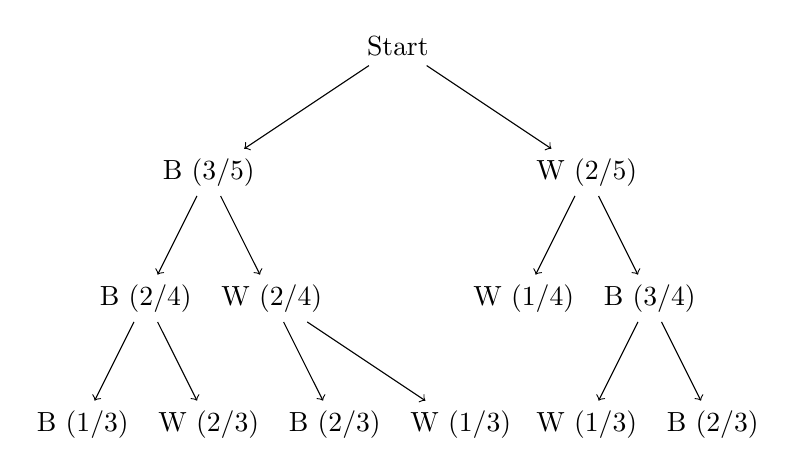
\begin{tikzpicture}[scale=0.8]
            % First draw
            \node (start) at (0,0) {Start};
            \node (B1) at (-3,-2) {B (3/5)};
            \node (W1) at (3,-2) {W (2/5)};
            \draw[->] (start) -- (B1);
            \draw[->] (start) -- (W1);

            % Second draw after first black
            \node (B2a) at (-4,-4) {B (2/4)};
            \node (W2a) at (-2,-4) {W (2/4)};
            \draw[->] (B1) -- (B2a);
            \draw[->] (B1) -- (W2a);

            % Second draw after first white
            \node (B2b) at (4,-4) {B (3/4)};
            \node (W2b) at (2,-4) {W (1/4)};
            \draw[->] (W1) -- (B2b);
            \draw[->] (W1) -- (W2b);

            % Third draw after second black
            \node (B3a) at (-5,-6) {B (1/3)};
            \node (W3a) at (-3,-6) {W (2/3)};
            \draw[->] (B2a) -- (B3a);
            \draw[->] (B2a) -- (W3a);

            % Third draw after second white
            \node (B3b) at (-1,-6) {B (2/3)};
            \node (W3b) at (1,-6) {W (1/3)};
            \draw[->] (W2a) -- (B3b);
            \draw[->] (W2a) -- (W3b);

            % Third draw after second black from first white
            \node (B3c) at (5,-6) {B (2/3)};
            \node (W3c) at (3,-6) {W (1/3)};
            \draw[->] (B2b) -- (B3c);
            \draw[->] (B2b) -- (W3c);
        \end{tikzpicture}
    \end{center}
    The probability of drawing 3 black marbles in a row is calculated by multiplying the probabilities along the branches leading to that outcome:
    \[
        P(\text{3 black}) = \frac{3}{5} \cdot \frac{2}{4} \cdot \frac{1}{3} = \frac{1}{10}
    \]
\end{eg}

\begin{eg}[Monty Hall Problem]
    In a game show, a contestant is presented with three doors: behind one door is a car (the prize), and behind the other two doors are goats. The contestant picks one door. The host, who knows what is behind each door, opens one of the remaining doors, revealing a goat. The contestant is then given the option to switch their choice to the other unopened door or stick with their original choice. What should the contestant do to maximize their chances of winning the car? \\
    Let's define the events:
    \begin{itemize}[itemsep=1pt,label=$\circ$]
        \item $C$ = "The car is behind the initially chosen door"
        \item $S$ = "The contestant switches doors"
    \end{itemize}
    The probability of winning the car if the contestant sticks with their original choice is:
    \[
        P(\text{win} | \text{stick}) = P(C) = \frac{1}{3}
    \]
    If the contestant switches doors, the probability of winning the car is:
    \[
        P(\text{win} | S) = P(\bar{C}) = \frac{2}{3}
    \]
    Therefore, to maximize their chances of winning the car, the contestant should always switch doors.
\end{eg}

\section{Random Variables}
Often e are not interested in the outcomes of an experiment per se, but some function of those outcomes. For examples:
\begin{itemize}[itemsep=1pt,label=$\circ$]
    \item The sum of the values of two dices.
    \item The money we win when rolling two dices summing up to 7.
    \item The number of $6$ we roll in $10$ rolls.
    \item The grade we obtain in an exam when guessing the answers.
\end{itemize}

\begin{definition}
    A random variable $X$ is a function $X: S \to \mathbb{R}$ from the sample space $S$ of an experiment to the set of real numbers $\mathbb{R}$. (note that it is not a variable in the usual sense, but rather a mapping and it is not random either).
\end{definition}

\begin{eg}
    Suppose that a coin is flipped three times. Let the sample space be:
    \[
        S = \{HHH, HHT, HTH, HTT, THH, THT, TTH, TTT\}
    \]
    Define the random variable \( X \) as the number of heads obtained in the three flips. The mapping of \( X \) is as follows:
    \begin{itemize}[itemsep=1pt,label=$\circ$]
        \item \( X(HHH) = 3 \)
        \item \( X(HHT) = 2 \)
        \item \( X(HTH) = 2 \)
        \item \( X(HTT) = 1 \)
        \item \( X(THH) = 2 \)
        \item \( X(THT) = 1 \)
        \item \( X(TTH) = 1 \)
        \item \( X(TTT) = 0 \)
    \end{itemize}
\end{eg}

\subsection{Random Variables vs. Events}
In the context of a random variable \( X \), events can be expressed in terms of the values that \( X \) takes. For example, if we are interested in the event that \( X \) takes on a specific value \( x \), we can denote this event as:
\[    E_x = \{ s \in S : X(s) = x \} \]
This event \( E_x \) consists of all outcomes in the sample space \( S \) for which the random variable \( X \) equals \( x \). This can be denoted as:
\[    P(X = x) = P(E_x)
\]
Note that instead of $=$, we could also use other relational operators such as \( <, \leq, >, \geq \) to define events based on the values of the random variable \( X \).

\begin{eg}
    Consider the same example as above where a coin is flipped three times and the random variable \( X \) represents the number of heads obtained.
    \[
        \begin{array}{cccc}
            \\ \text{Event} & \text{Outcomes} & \text{Meaning} & \text{Probability Statement} \\ \\
            \hline \\
            X = 1 & \{HTT, THT, TTH\} & X \text{ takes on the value } 1 & P(X = 1) \\ \\
            X < 2 & \{HTT, THT, TTH, TTT\} & X \text{ takes on values $0$ or $1$ } & P(X < 2) \\ \\
            X \geq 2 & \{HHT, HTH, THH, HHH\} & X \text{ takes on values $2$ or $3$ } & P(X \geq 2) \\ \\
            X = x & \ldots & X \text{ takes on the value } x & P(X = x) \\ \\
        \end{array}
    \]
\end{eg}

\subsection{Distribution of a Random Variable}

\begin{definition}[Distribution]
    The distribution of a random variable $X$ on a sample space $S$ is the list of all possible values $r$ that $X$ can take on together with the probabilities $P(X = r)$ for all $r \in X(S)$ where $P(X = r)$ is the probability that $X$ takes the value $r$.
    \[
        P(X = r) = \sum_{s \in S : X(s) = r} P(s)
    \]
\end{definition}
Remark that:
\begin{itemize}[itemsep=1pt,label=$\circ$]
    \item If the range of the function $X$ is countable, then $P(X = r)$ can be interpreted as a function $P: X(S) \to \mathbb{R}$.
    \item This function $P$ is called the probability mass function (PMF) and it is a probability distribution over the sample space $X(S)$.
\end{itemize}
Note that in this class, we will only consider this case:
\[
    \sum_{r \in X(S)} P(X = r) = \sum_{r \in X(S)} \sum_{s \in S : X(s) = r} P(s) = \sum_{s \in S} P(s) = 1
\]

\begin{eg}
    Consider that two fair dice are rolled. Let the random variable \( X \) be defined as the sum of the numbers appearing on the two dice. The possible values of \( X \) range from \( 2 \) to \( 12 \). The distribution of \( X \) is as follows:
    \[
        \begin{array}{c|c}
            \text{Value of } X & P(X = r) \\ \hline
            2 & \frac{1}{36} \\
            3 & \frac{2}{36} \\
            4 & \frac{3}{36} \\
            5 & \frac{4}{36} \\
            6 & \frac{5}{36} \\
            7 & \frac{6}{36} \\
            8 & \frac{5}{36} \\
            9 & \frac{4}{36} \\
            10 & \frac{3}{36} \\
            11 & \frac{2}{36} \\
            12 & \frac{1}{36} \\
        \end{array}
    \]
    Graphically, the distribution can be represented as follows:
    \begin{center}
        \begin{tikzpicture}[scale=1]
            \draw[->] (-3.5,0) -- (3.5,0) node[right] {$x$};
            % \draw[->] (0,-3) -- (0,3) node[above] {$y$};

            \foreach \x in {2,3,4,5,6,7,8,9,10,11,12} {
                \ifnum\x>7\relax
                    \pgfmathsetmacro{\yt}{13-\x}
                    \pgfmathsetmacro{\y}{(1/36)*\yt*15} % Calculate the height based on the distribution
                \else
                    \pgfmathsetmacro{\yt}{\x-1}
                    \pgfmathsetmacro{\y}{(1/36)*\yt*15} % Calculate the height based on the distribution
                \fi

                % \pgfmathsetmacro{\y}{(1/36)*(\x-1)*10} % Calculate the height based on the distribution
                \draw[fill=secondary] (\x-7,-0.1) rectangle (\x-6,\y); % Draw the bar
                \node[above] at (\x-6.5,\y+0.3) {$\frac{\pgfmathprintnumber[fixed,precision=0]{\yt}}{36}$}; % Label the height with a int precision of 0 decimal
                \node[below] at (\x-6.5,-0.3) {\x}; % Label the x-axis
            }
        \end{tikzpicture}
    \end{center}
\end{eg}

\begin{eg}
    Suppose that a coin is flipped three times. Let $X(s)$ be the random variable that equals the number of heads that appear when $s$ is the outcome. What is the probability of $P(X = 1)$? \\
    The sample space is:
    \[
        S = \{HHH, HHT, HTH, HTT, THH, THT, TTH, TTT\}
    \]
    The outcomes where \( X = 1 \) are:
    \[
        E = \{HTT, THT, TTH\}
    \]
    Therefore:
    \[
        P(X = 1) = P(E) = \frac{3}{8}
    \]
\end{eg}
Note this example could be solved using Bernoulli Trials where \( n = 3 \), \( k = 1 \), and \( p = \frac{1}{2} \):
\[
    P(X = 1) = \binom{3}{1} \left(\frac{1}{2}\right)^1 \left(\frac{1}{2}\right)^{3-1} = 3 \cdot \frac{1}{2} \cdot \frac{1}{4} = \frac{3}{8}
\]
Thus generalized, the number of successes $k$ in \( n \) Bernoulli trials with probability of success \( p \) is a random variable \( X \) with distribution:
\[
    P(X = k) = \binom{n}{k} p^k (1 - p)^{n - k}
\]

\subsection{Expected Value}
\begin{definition}[Expected Value]
    The expected value (or mean) of a discrete random variable \( X \) on the sample space $S$ is equal to:
    \[
        E(X) = \sum_{s \in X(S)} P(s) \cdot X(s) = \sum_{r \in X(s)} \left(\sum_{s \in S : X(s) = r} P(s) \cdot X(s)\right) = \sum_{r \in X(S)} P(X = r) \cdot r
    \]
\end{definition}

\begin{eg}
    Let $X$ be the number of points obtained in a multiple choice question with $1$ correct answer out of $4$ options. Choosing the correct option results in $1$ point, while choosing one of the incorrect options will result in $-\frac{1}{3}$ points. What is the expected number of points when guessing? \\
    The possible outcomes for \( X \) are:
    \[
        X(S) = \left\{ 1, -\frac{1}{3} \right\}
    \]
    The probabilities are:
    \[
        P(X = 1) = \frac{1}{4}, \quad P\left(X = -\frac{1}{3}\right) = \frac{3}{4}
    \]
    Therefore, the expected value of \( X \) is:
    \[
        E(X) = P(X = 1) \cdot 1 + P\left(X = -\frac{1}{3}\right) \cdot \left(-\frac{1}{3}\right) = \frac{1}{4} \cdot 1 + \frac{3}{4} \cdot \left(-\frac{1}{3}\right) = \frac{1}{4} - \frac{1}{4} = 0
    \]
\end{eg}